\subsection{A slower decline in the AI-service price}
\label{subsec:rewrite-rsi-half-decline}

I repeat the RSI-activation exercise with a price decline half as large as
the rounded observed decline. At $\sigma=1$, I now calibrate $\chi$ to
\begin{equation}
 \frac{p_X(2.25)}{p_X(0)}=1-\frac{0.80}{2}=0.60.
 \label{eq:rewrite-rsi-half-price-target}
\end{equation}
The target is a $40\%$ decline over 2.25 years, rather than $80\%$.
It halves the percentage decline, not its logarithm, the annual growth
rate, or $\chi$ itself. This is an illustrative sensitivity exercise,
not a second empirical estimate or an estimate of how monopoly changes
the pace of price declines.

At unit elasticity, Equation~\eqref{eq:rewrite-monopoly-foc} gives a
constant markup and a price inversely proportional to $B$. The original
target therefore requires $B$ to increase fivefold within 2.25 years;
the new target requires an increase by a factor of $5/3$. Halving the
percentage price decline does not halve the required efficiency gain.

All other parameters and initial stocks are unchanged. Each economy starts
on the same fixed-efficiency BGP as in
Section~\ref{subsec:rewrite-rsi-activation}, with existing AI and
$K_0/Y_0=3.30$. RSI is activated unexpectedly at date zero. I recalibrate
$\chi$ at unit elasticity, hold it fixed across the other three elasticities,
and solve consumption and research again using the same BVP and equilibrium
checks. The new paths are not time-rescaled versions of the earlier paths.
Table~\ref{tab:rewrite-rsi-half-parameters} reports the parameters and initial stocks.

\begin{rewriteParameterTable}{Faster-transition sensitivity: parameters and initial stocks}{tab:rewrite-rsi-half-parameters}
$\omega_X$ & 0.10 & AI production weight & Same assumed value as in Table~\ref{tab:rewrite-research-share-parameters}; not fitted to industry size.\\
$\omega_L$ & 0.90 & Effective-labor weight & Computed as $1-\omega_X$.\\
$\chi$ & 7.616305 & Research productivity after activation & Fitted at $\sigma=1$ to Equation~\eqref{eq:rewrite-rsi-half-price-target}; common across elasticities.\\
$\sigma$ & 0.90; 1; 1.10; 1.50 & AI--labor substitution & Same arbitrary scenarios.\\
$\overline B$ & 1,360.992139 & AI-efficiency upper bound & $1.10\mathcal B(1.50)$; unchanged arbitrary margin above the threshold.\\
\midrule
$A_0,N_0$ & 1; 1 & Initial technology and population & Same unit normalizations.\\
$B_0$ & 13.609921 & Initial AI efficiency & $0.01\overline B$; same arbitrary initial distance.\\
$K_0$ & 3.433645; 4.649320; 5.036956; 5.504667 & Initial capital, by $\sigma$ & Same fixed-efficiency BGP stocks with existing AI; Equation~\eqref{eq:rewrite-rsi-initial-ratio}.\\
$K_0/Y_0$ & 3.30 & Initial capital--output ratio & Same pre-RSI BGP ratio, preserved at activation.\\
\end{rewriteParameterTable}

The fitted value is $\chi=7.616305$, about $20.7\%$ of the value in the
preceding exercise. Initial output-per-person growth is now $1.62\%$,
$2.71\%$, $3.02\%$, and $4.54\%$ across the four elasticities. In particular,
at $\sigma=1.50$ it falls from $23.97\%$ to $4.54\%$. Output, wages, and
prices remain continuous at activation; their growth rates can still adjust
immediately. The smaller price decline produces a less abrupt transition,
not a fully smooth activation.

The initial resource reallocation is also smaller. At $\sigma=1.50$,
consumption rises by $5.05\%$ at activation instead of $22.71\%$, and
research absorbs $3.10\%$ of output instead of $9.32\%$. The developer's
initial net profit is positive, at $0.20\%$ of output, compared with a loss
of $6.02\%$ in the preceding exercise. Gross investment is $13.79\%$ of
output rather than $-6.09\%$. This calibration therefore requires neither
an initial developer loss nor negative gross investment. Investment remains
below depreciation, however, so the capital stock initially falls at an
annualized rate of $0.82\%$. These are equilibrium outcomes, not added
financing or investment constraints.

The distributional transition takes longer. At $\sigma=1.50$, labor's
income share reaches half its initial value after approximately $46.8$
years, compared with $11.7$ years in the preceding exercise. It completes
$90\%$ of its decline toward zero after about $137$ years rather than $60$.
The long-run growth rates, interest rates, and income shares are unchanged:
lower research productivity changes the transition, not the regime selected
by the production parameters and the AI-efficiency upper bound.
The initial size of the AI industry is also unchanged and remains an
unfitted feature of the calibration.


Figures~\ref{fig:rewrite-rsi-half-accumulation}--\ref{fig:rewrite-rsi-half-distribution}
retain the variables, normalizations, line styles, and time windows of the
preceding exercise. Vertical scales may differ between exercises to keep
the individual paths legible. Dotted horizontal lines show the unchanged
analytical limits for $\sigma=1.50$.

\begin{figure}[H]
 \centering
 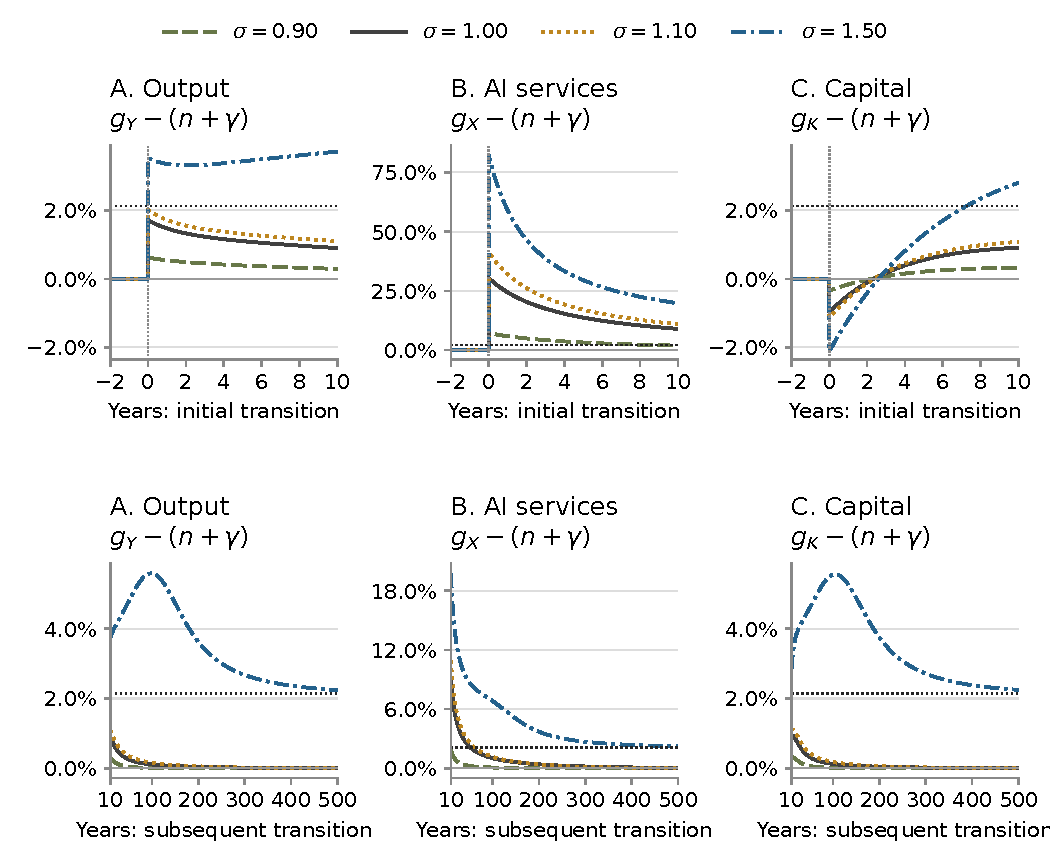
\includegraphics[width=\textwidth]{figures_rewrite/equilibrium_rsi_activation_half_decline_accumulation_growth_windows.pdf}
 \caption{A $40\%$ price-decline target: growth of output, AI production
 services, and capital per unit of effective labor. Rates are instantaneous
 annual rates. The upper row shows two pre-event years and years 0--10;
 the lower row shows years 10--500. Panels A and C share a scale within
 each row. The vertical line marks RSI activation.}
 \label{fig:rewrite-rsi-half-accumulation}
\end{figure}

\begin{figure}[H]
 \centering
 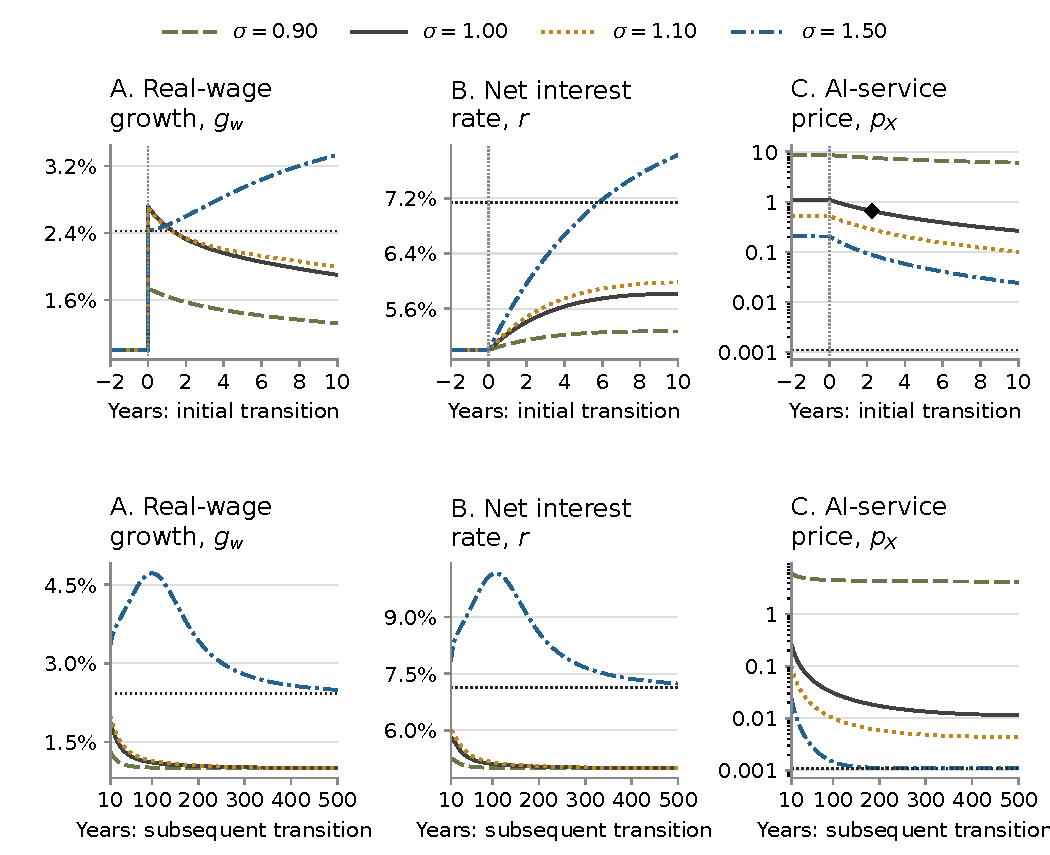
\includegraphics[width=\textwidth]{figures_rewrite/equilibrium_rsi_activation_half_decline_growth_returns_windows.pdf}
 \caption{A $40\%$ price-decline target: real-wage growth, the net interest
 rate, and the AI-service price. Rates are annual; the price is in final-good
 units on a logarithmic scale. The diamond marks the unit-elastic target
 $p_X(2.25)/p_X(0)=0.60$. The vertical line marks RSI activation.}
 \label{fig:rewrite-rsi-half-prices}
\end{figure}

\begin{figure}[H]
 \centering
 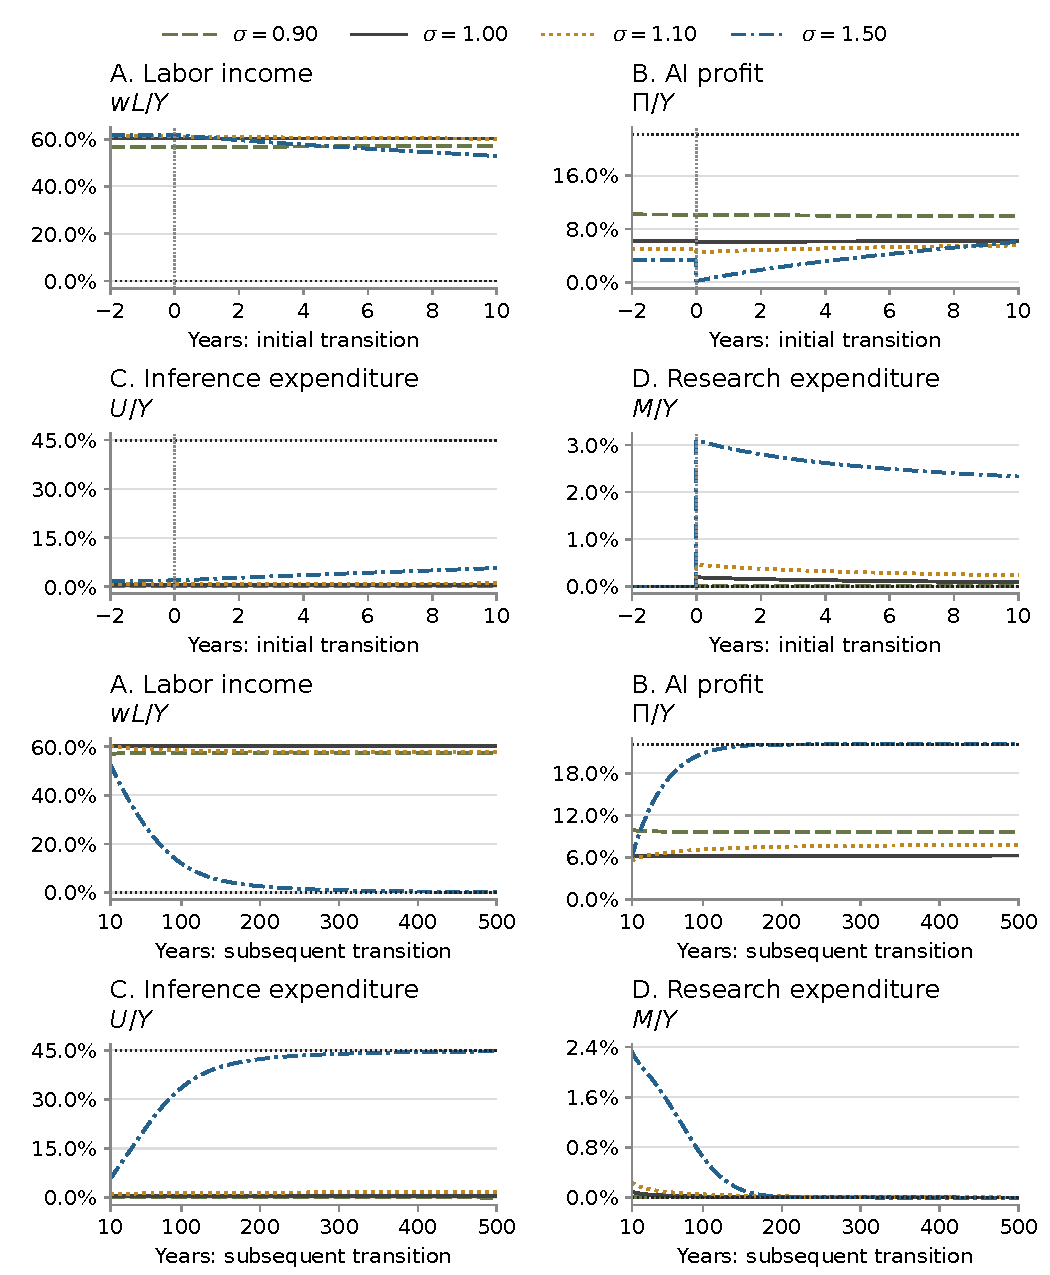
\includegraphics[width=\textwidth]{figures_rewrite/equilibrium_rsi_activation_half_decline_ai_distribution_windows.pdf}
 \caption{A $40\%$ price-decline target: labor income, AI net profit,
 inference expenditure, and research expenditure relative to output.
 The first two rows show the pre-event BGP and years 0--10; the last two
 show years 10--500. The omitted gross capital share remains $\alpha=0.33$.}
 \label{fig:rewrite-rsi-half-distribution}
\end{figure}
